
\documentclass[10 pt,usenames,dvipsnames, oneside]{article}
\usepackage{../../modelo-fracoes}
\graphicspath{{../../../Figuras/licao04/}}


\begin{document}

\begin{center}
  \begin{minipage}[l]{3cm}
\includegraphics[width=2cm]{../../../Figuras/logo}       
\end{minipage}\hfill
\begin{minipage}[r]{.8\textwidth}
 {\Large \scshape Atividade: Discos de frações - quantos cabem?}  
\end{minipage}
\end{center}
\vspace{.2cm}

\ifdefined\prof
%Caixa do Para o Professor
\begin{goals}
%Objetivos específicos
\begin{enumerate}
\item       Reconhecer que as frações       $\frac{2}{3}$,
$\frac{4}{6}$       e       $\frac{8}{12}$       são iguais a partir da
observação das representações destas frações em modelos de área circulares.
\end{enumerate}

\tcblower

%Orientações e sugestões
\begin{itemize}
\item       Recomenda-se que esta atividade seja desenvolvida em grupos de
$2$       ou       $3$       alunos para que eles possam discutir as
soluções apresentadas, dentro do grupo, durante a condução da atividade.
\item       Os setores circulares empregados na condução da atividade podem
ser aproveitados da \hyperref[chap1-ativ10]{Atividade \ref{chap1-ativ10}} da Lição 1.
\item       É importante, ao final da atividade, observar para os alunos que
uma mesma parte do círculo (a área da região pintada de cinza) está sendo
descrita por frações com numeradores e denominadores diferentes (isto é, por
frações equivalentes), mas que, não obstante, por expressarem uma mesma
quantidade, estas frações são iguais, não apenas porque por sobreposição parecem
ser a mesma quantidade, mas porque, como na atividade anterior, se cada terço do
círculo for subdividido em 2 e 4 partes iguais, respectivamente, então, de fato,
$\frac{2}{3}$       =       $\frac{4}{6}$       e       $\frac{2}{3}$
=       $\frac{8}{12}$.
\item       Além disso, observaçào análoga cabe para as frações que
completam a terceira coluna da tabela:       $\frac{1}{3}$       =
$\frac{2}{6}$       e       $\frac{1}{3}$       =       $\frac{4}{12}$.
\end{itemize}
\end{goals}

\bigskip
\begin{center}
{\large \scshape Atividade}
\end{center}
\fi

O objetivo desta atividade é estudar a fração do círculo que está pintada de cinza no encarte que você recebeu.

\begin{center}
 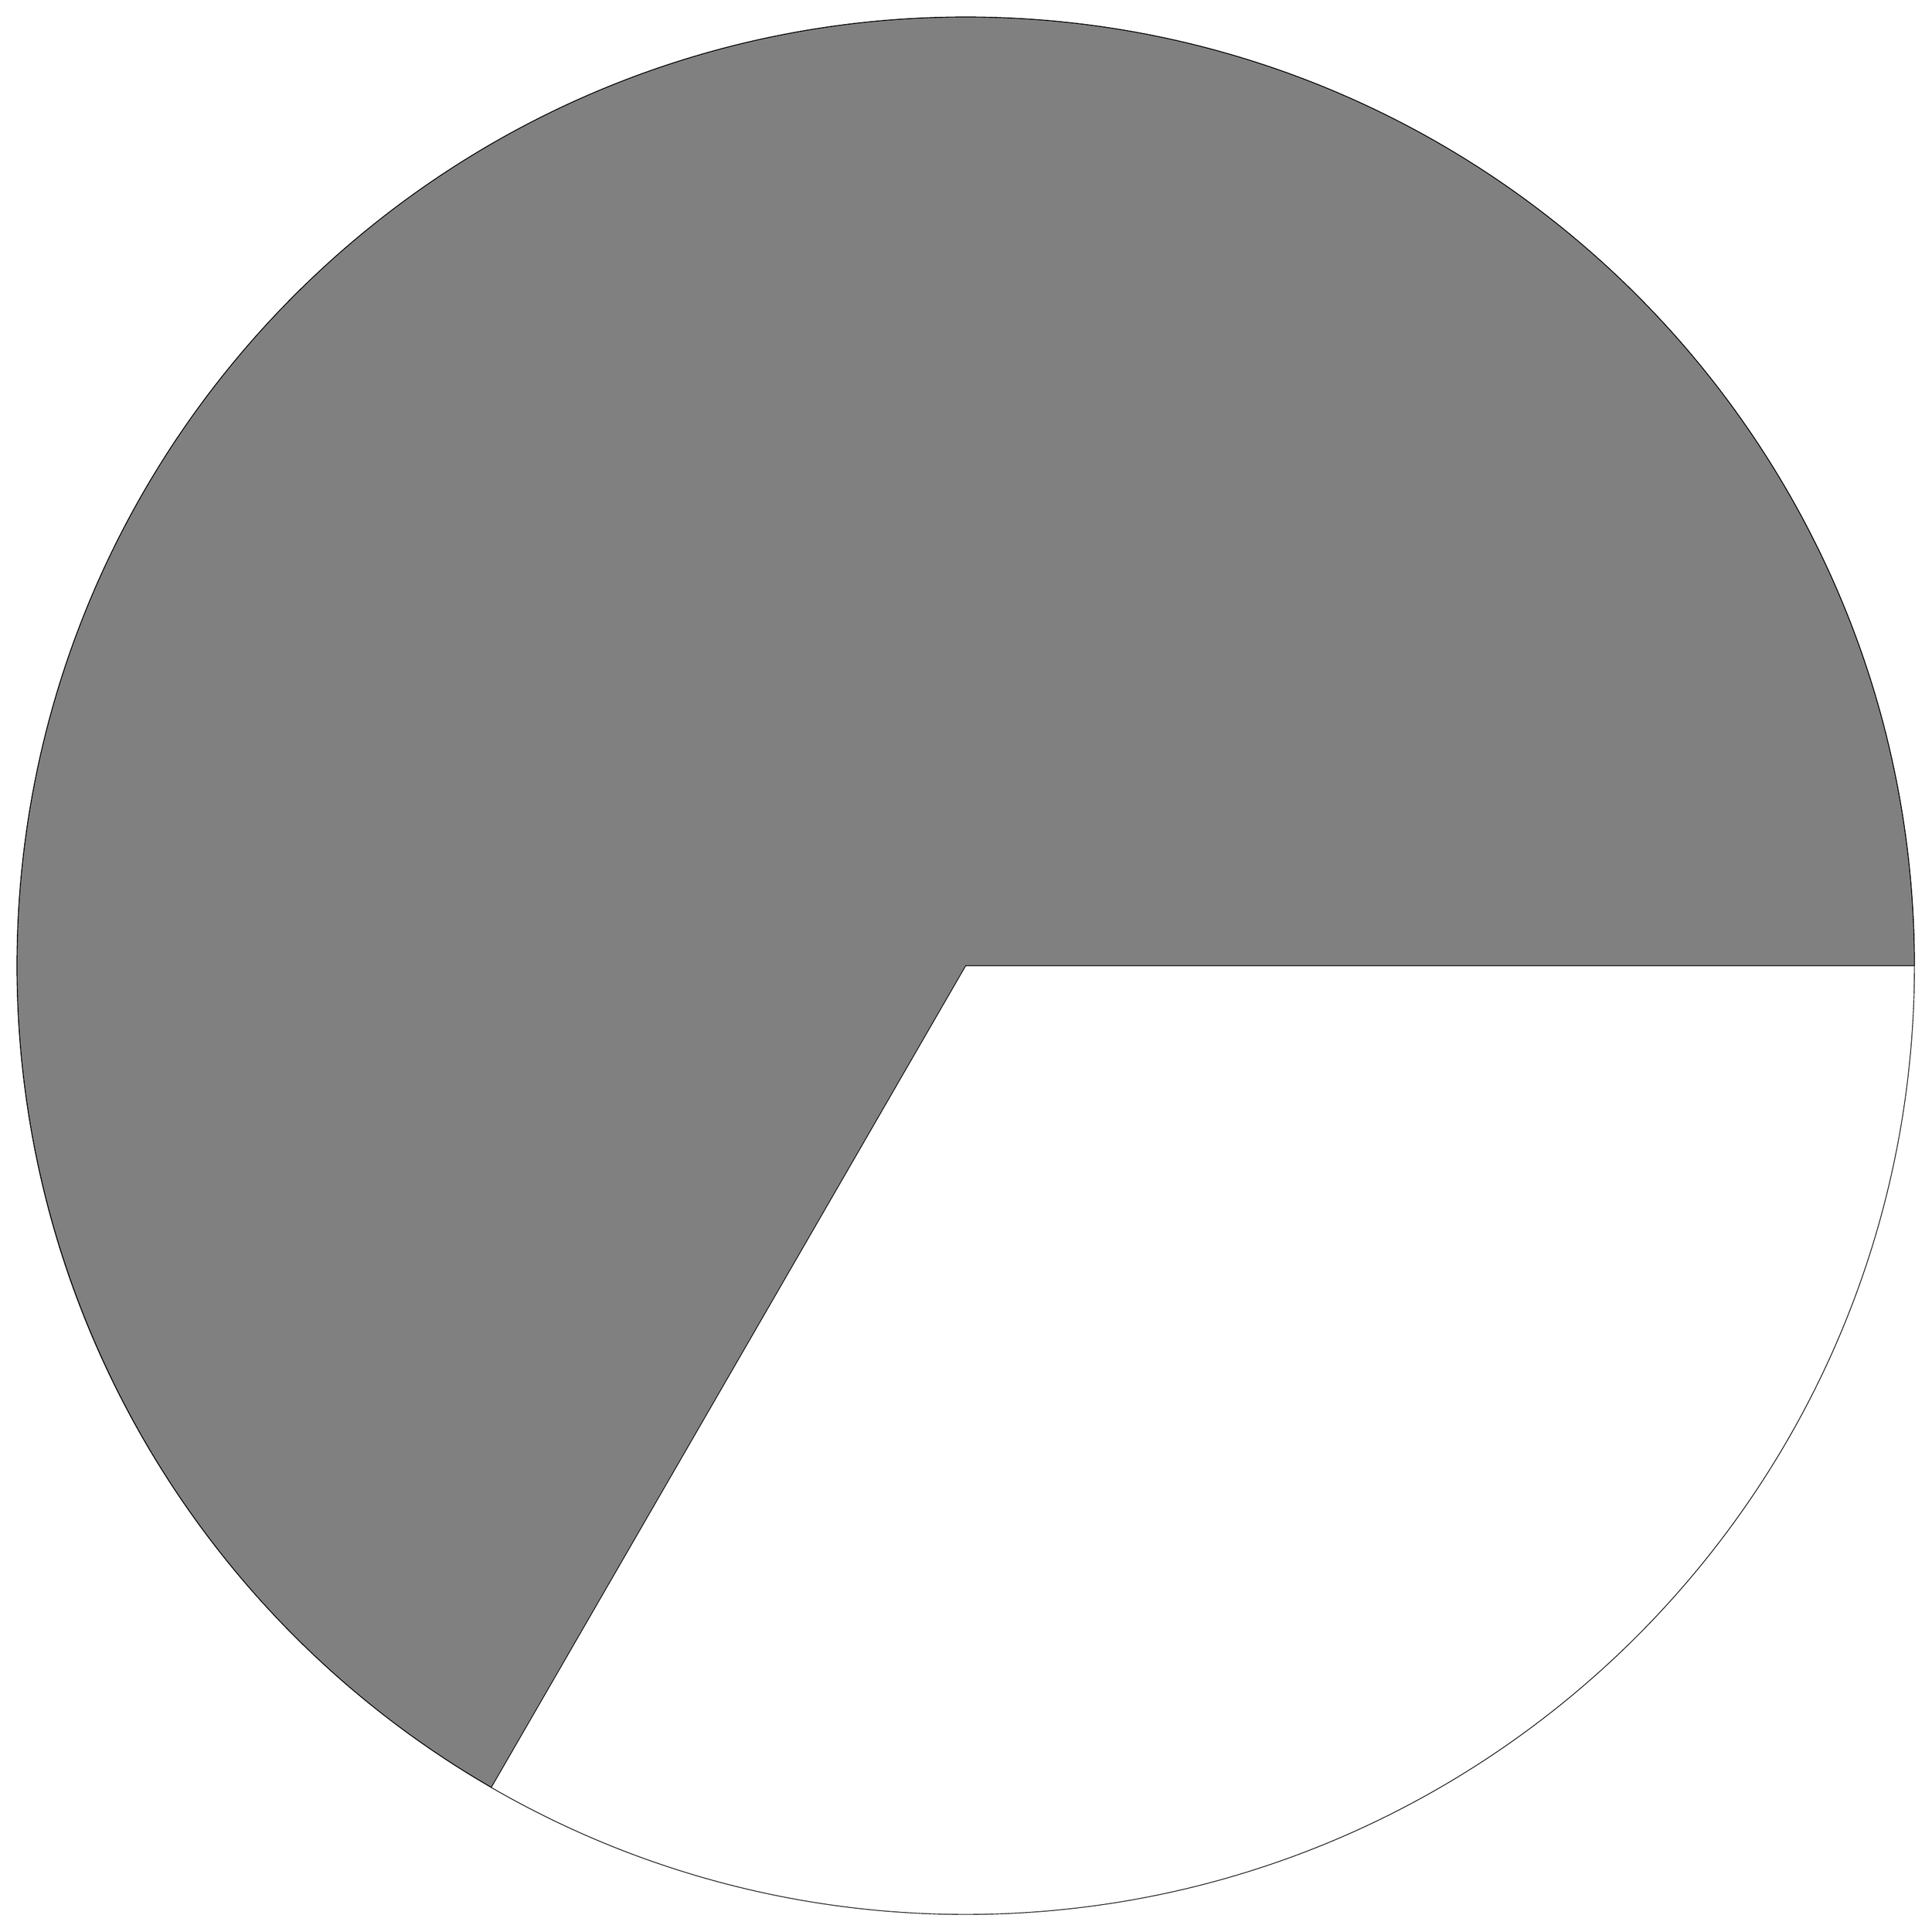
\begin{tikzpicture}
  \draw[fill=gray] (20,0) arc (0:240:20) -- (0,0)--cycle;
  \draw (0,0) circle (20);
 \end{tikzpicture}
\end{center}

Para isto, responda às perguntas na tabela a seguir com frações adequadas. Se necessário, use as peças coloridas que você recortou e usou na \hyperref[chap1-ativ10]{Atividade 10 da Lição 1} para avaliar as suas respostas.

  \noindent \begin{longtable}{|m{0.25\textwidth}|m{0.2\textwidth}|m{0.2\textwidth}|m{0.2\textwidth}|}
    \hline
     Tipo da peça &   Quantas peças como essa cabem na região cinza? &   As peças que você usou, juntas, são que fração do círculo?  &  Que fração do círculo não está colorida de cinza? \\
    \hline
    \endhead
     $\frac{1}{3}$
\begin{center}
 \begin{tikzpicture}[scale=.8]
  \draw[fill=common] (20,0) arc (0:120:20) -- (0,0)--cycle;
 \end{tikzpicture}
\end{center}
     &  &  &  \\
    \hline
     $\frac{1}{6}$
\begin{center}
\begin{tikzpicture}[scale=.8]
  \draw[fill=light] (20,0) arc (0:60:20) -- (0,0)--cycle;
\end{tikzpicture}
\end{center}
     &  &  &  \\
    \hline
     $\frac{1}{12}$
\begin{center}
\begin{tikzpicture}[scale=.8]
  \draw[fill=special] (20,0) arc (0:30:20) -- (0,0)--cycle;
\end{tikzpicture}
 \end{center}
&  &  &  \\
    \hline
  \end{longtable}

\ifdefined\prof
\begin{solucao}

\vspace{1em}
\noindent\begin{tabular}{|m{0.25\textwidth}|m{0.22\textwidth}|m{0.2\textwidth}
|m{0.2\textwidth}|}
\hline
Tipo da peça &   Quantas cabem na região cinza? &   Juntas, são que fração
do círculo?  &  Fração do círculo não colorida de cinza? \\
\hline
$\frac{1}{3}$
\begin{center}
\begin{tikzpicture}[x=1mm,y=1mm,scale=.5]
\draw[fill=common] (20,0) arc (0:120:20) -- (0,0)--cycle;
\end{tikzpicture}
\end{center}
& $2$ &  $\frac{2}{3}$ &  $\frac{1}{3}$ \\
\hline
$\frac{1}{6}$
\begin{center}
\begin{tikzpicture}[x=1mm,y=1mm,scale=.5]
\draw[fill=light] (20,0) arc (0:60:20) -- (0,0)--cycle;
\end{tikzpicture}
\end{center}
&  $4$ &  $\frac{4}{6}$ &  $\frac{2}{6}$ \\
\hline
$\frac{1}{9}$
\begin{center}
\begin{tikzpicture}[x=1mm,y=1mm,scale=.5]
\draw[fill=special] (20,0) arc (0:40:20) -- (0,0)--cycle;
\end{tikzpicture}
\end{center}
&   $6$ &  $\frac{6}{9}$ &  $\frac{3}{9}$ \\
\hline
\end{tabular}

\end{solucao}
\fi

\end{document}